\begin{slide}
\pagestyle{headings}
\sf
%
\vspace*{-4mm}
\header{Straight line fit}
\vspace{5mm}
\Large 
\sf
\begin{figure}[h]
\unitlength1cm 
  \begin{picture}(8,5.)
    \put(7.,-1.){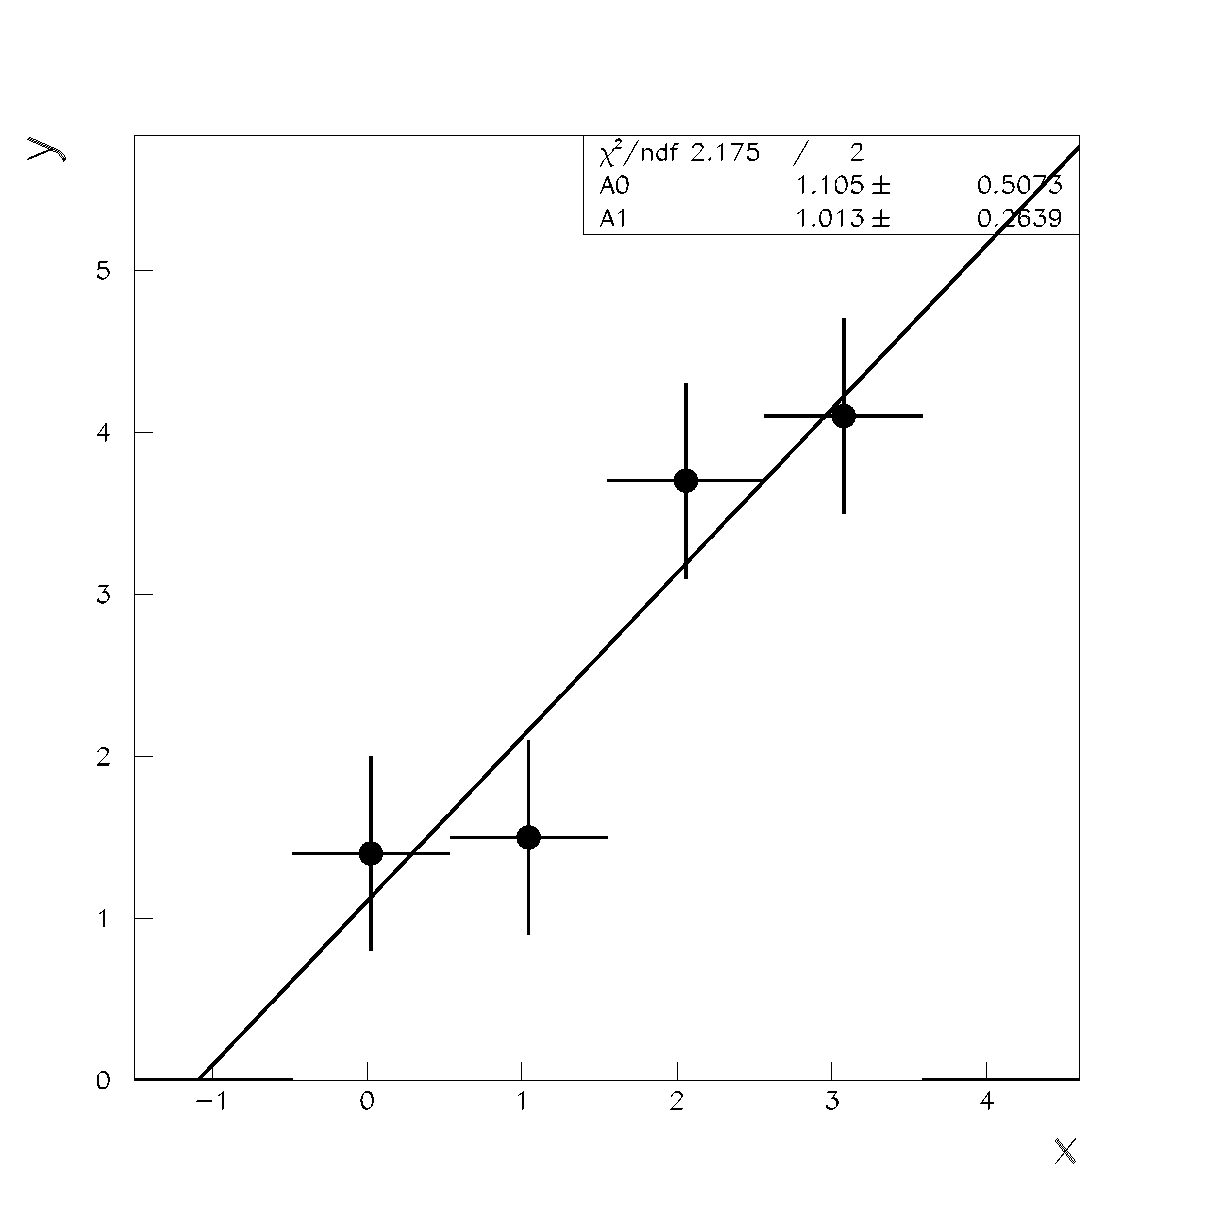
\epsfig{file=eps/p1.eps,width=7.cm}}
\put(0.,2.5){
\begin{minipage}{6.3cm}
\large \sf
{\bfseries Model: $\pmb{y = a_0 + a_1 x }$}\\[1mm]
Simple example: All $y_i$ have the same uncertainty and
are uncorrelated
\[  
V = \left(
\begin{array}{lll}
\sigma^2 &    &    0 \\
         & .  &      \\
0        &    &    \sigma^2 \\
\end{array}
\right) 
 \]
\[ \chi^2 = \sum_{i=1}^n \frac{\dd (y_i - a_0 - a_1\, x_i)^2}{\dd \sigma^2} \]

\end{minipage}
}
\end{picture}
\end{figure}


\large \sf
\vspace{4mm}

Matrix notation: $ \vec{y} = A\vec{a}; \qquad 
\vec{a} 
\left(
\begin{array}{l}
a_0\\
a_1\\
\end{array}
\right)
\quad
A = 
\left( 
\begin{array}{ll}
  1 & x_1 \\
  . & .   \\
  1 & x_n \\
 \end{array}
\right)
, \quad 
A^T = 
\left(
\begin{array}{lll}
    1 & ... & 1   \\
  x_1 & ... & x_n \\
\end{array}
\right)
$
\begin{eqnarray*} 
 \hat{\vec{a}} & =  & \left( 
\begin{array}{l}
\hat{a}_0 \\
\hat{a}_1 \\
 \end{array}
\right)
= ( A^T V^{-1} A )^{-1} A^T V^{-1} \vec{y}
; \qquad V^{-1} = 
\left(
\begin{array}{lll}
1/\sigma^2 &    &    0 \\
         & .  &      \\
0        &    &    1/\sigma^2 \\
\end{array}
\right) 
\\
\end{eqnarray*}
\end{slide}
%
%
%
\begin{slide}
\pagestyle{headings}
\sf
%
\header{Straight line fit}
%\vspace*{-5mm}
\begin{eqnarray*} 
 \hat{\vec{a}} 
 &  = &  \sigma^2 ( A^T A)^{-1} \cdot \frac{1}{\sigma^2} A^T\cdot \vec{y} 
\;  = \; (A^T A)^{-1} A^T \cdot \vec{y} 
\\
&  = & \left(
\begin{array}{ll}
\sum_{i} 1 & \sum_{i} x_i \\
. & . \\
\sum_{i} x_i & \sum_{i} x_i^2 \\
\end{array}
\right)^{-1} \cdot 
\left( 
\begin{array}{l}
\sum_{i} y_i \\
\sum_{i} x_i y_i \\
\end{array}
\right)
\; 
 =\;  \left(
\begin{array}{ll}
N & N \overline{x} \\
N \overline{x} & N \overline{x^2} \\
\end{array}
\right)^{-1} 
\cdot \left( 
\begin{array}{l} 
N\overline{y} \\
N\overline{xy} \\
\end{array}
\right) 
\\
&  =  & \left(
\begin{array}{ll}
1 & \overline{x} \\
\overline{x} & \overline{x^2} \\
\end{array}
\right)^{-1} \cdot 
\left( 
\begin{array}{l} 
\overline{y}\\
\overline{xy}\\
\end{array}
\right)
\; 
 = 
\; 
\frac{1}{\overline{x^2} - \overline{x}^2} 
\left(
\begin{array}{lr} 
\overline{x^2} & -\overline{x} \\
-\overline{x} & 1 \\
\end{array}
\right) 
\left( \begin{array}{l}
\overline{y}\\
\overline{xy} 
\end{array}
\right) 
%\\[4mm]
%&  = &  
= 
\frac{1}{V[x]} \cdot
\left( 
\begin{array}{l} 
\overline{x^2} \overline{y} - \overline{x}\, \overline{xy} \\
-\overline{x}\,\overline{y} + \overline{xy} \\
\end{array}
\right) 
\end{eqnarray*}
Covariance matrix:
\[ \pmb{U} = \left(
\begin{array}{ll}
\sigma_{a_0}^2 & cov(a_0,a_1) \\
cov(a_0,a_1) & \sigma_{a_1}^2 \\
\end{array}
\right)  = (A^t V^{-1} A )^{-1} = \pmb{\frac{\sigma^2}{N V[x]} 
\left( \begin{array}{lr}
\overline{x^2} & -\overline{x} \\
-\overline{x} & 1 \\
\end{array}
\right) 
}
\]
\end{slide}

%\vspace{2mm}
\begin{slide}
\Large
\pagestyle{headings}
\sf
\bheader{Mini exercise: straight line track-fit with N detectors}
%\renewcommand{\baselinestretch}{0.4}
%{\bfseries 
\noindent
The covariance formula 
\[ 
 \left(
\begin{array}{ll}
\sigma_{a_0}^2 & cov(a_0,a_1) \\
cov(a_0,a_1) & \sigma_{a_1}^2 \\
\end{array}
\right) = 
\frac{\sigma^2}{N V[x]}
\left( \begin{array}{lr}
\overline{x^2} & -\overline{x} \\
-\overline{x} & 1 \\
\end{array}
\right) 
\]
is valid for e.g. a straight line track fit  
in N detectors of resolution $\sigma$:

{
\darkgreen 
\bfseries \large
 Determine  
the improvements on the slope error  $\pmb{\sigma_{a_1}}$
by:
\begin{itemize}
\item[a)] 
Doubling the number of detector layers\\ within the same interval
in $\pmb{x}$
\item[b)] Distributing the detector layers\\ over an interval in
$\pmb{x}$ twice as large
\item[c)] 
Buying detectors with measurement uncertainties\\ reduced by a factor two
\end{itemize}
}
\end{slide}


\begin{slide}
\Large
\pagestyle{headings}
\sf
\bheader{\darkgreen{Mini-exercise} Straight-line fit example}
%
\begin{figure}[h]
\unitlength1cm
  \begin{picture}(8,8.)
    \put(0.,0.){\epsfig{file=eps/straightline.eps,width=7.cm}}
%    \put(-1.3,0.){\epsfig{file=eps/prob_examples.ps,width=7.cm}}

\put(0.,-1.){\normalsize see  $/afs/desy.de/user/m/mgoebel/public/StatisticsWS/StraightLineFit.C$}
\put(8.,7.){
\begin{minipage}[t]{7cm}
\darkgreen

Tasks: Do the fit, plot the error ellipse, get the 1-sigma band, judge
fit quality, etc. 
\end{minipage}
}
%\put(-.5,1.){\large \red $prob(\chi^2,n)$ vs $\chi^2$ for various $n$}
%\put(6.,3.){Add plot of expected flat distribution}
\end{picture}
\end{figure}
%
\end{slide}

\begin{slide}
\Large
\pagestyle{headings}
\sf
\bheader{\darkgreen{Mini-exercise} Real Trackfit in Si + driftchamber}
\vspace{4mm}
%
\begin{figure}[h]
\unitlength1cm
  \begin{picture}(8,8.)
    \put(-1.5,-1.){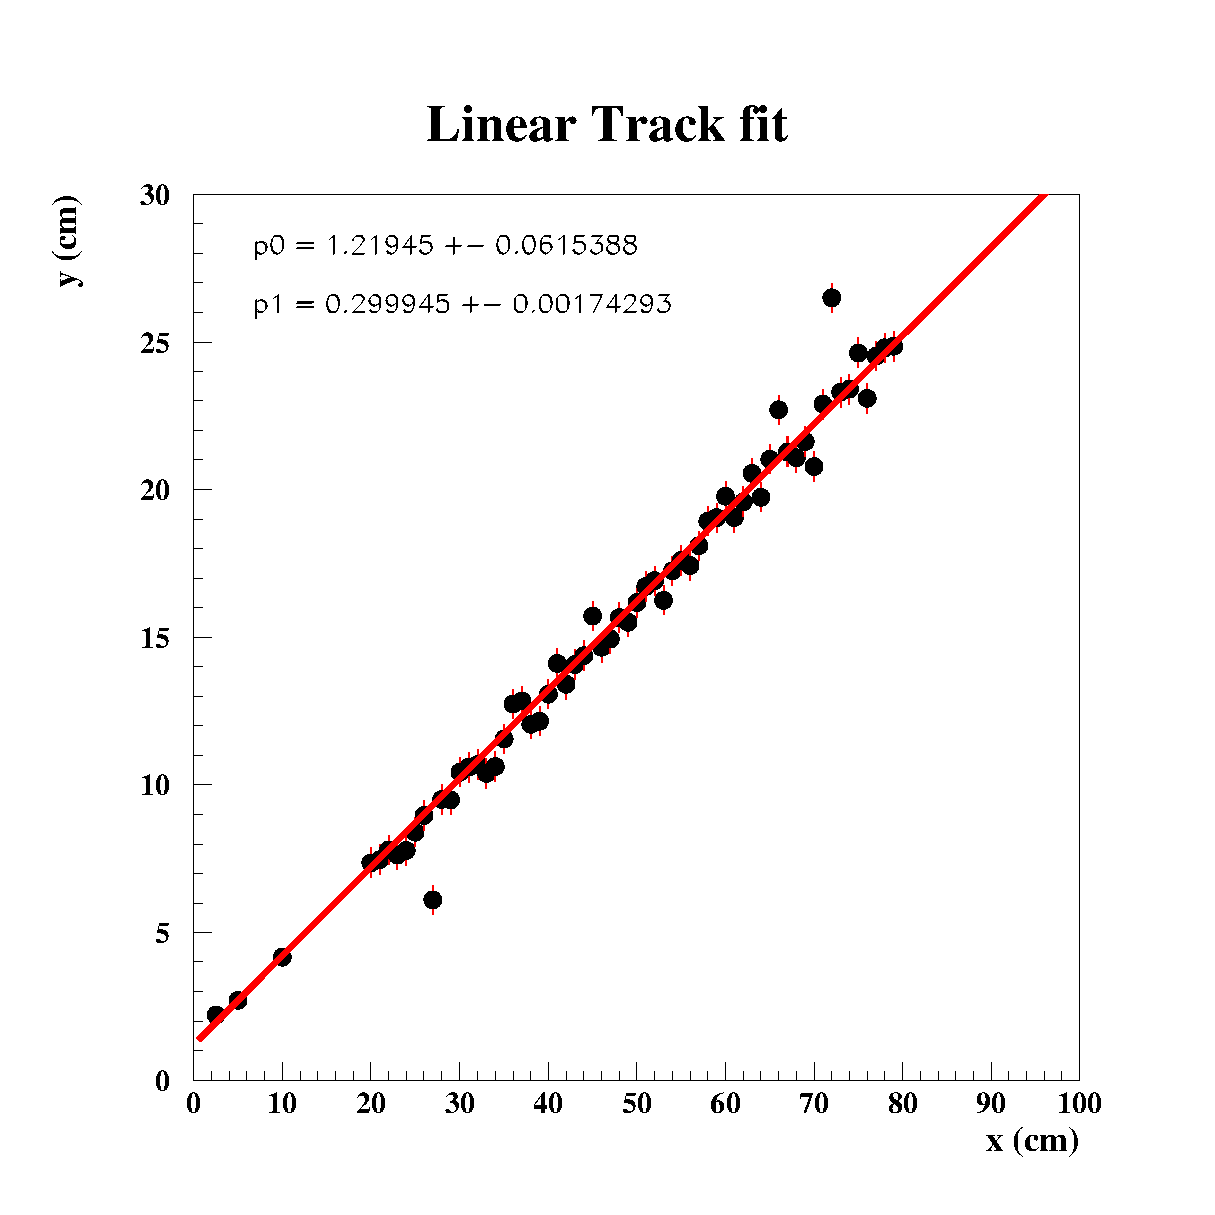
\epsfig{file=eps/trackfit.ps,width=10.cm}}
%    \put(-1.3,0.){\epsfig{file=eps/prob_examples.ps,width=7.cm}}
%\put(0.,-1.){\normalsize see  $/afs/desy.de/user/m/mgoebel/public/StatisticsWS/StraightLineFit.C$}
\put(8.,7.){
\begin{minipage}[t]{7cm}
\darkgreen

Tasks: Do the straight line fit, plot the error ellipse, get the 1-sigma band, judge
fit quality, reject outliers!, fit with parabola, determine momentum and error, 
extension: add vertex constraint 
\end{minipage}
}
%\put(-.5,1.){\large \red $prob(\chi^2,n)$ vs $\chi^2$ for various $n$}
%\put(6.,3.){Add plot of expected flat distribution}
\end{picture}
\end{figure}
%
\end{slide}
